
%% bare_conf.tex
%% V1.3
%% 2007/01/11
%% by Michael Shell
%% See:
%% http://www.michaelshell.org/
%% for current contact information.
%%
%% This is a skeleton file demonstrating the use of IEEEtran.cls
%% (requires IEEEtran.cls version 1.7 or later) with an IEEE conference paper.
%%
%% Support sites:
%% http://www.michaelshell.org/tex/ieeetran/
%% http://www.ctan.org/tex-archive/macros/latex/contrib/IEEEtran/
%% and
%% http://www.ieee.org/

%%*************************************************************************
%% Legal Notice:
%% This code is offered as-is without any warranty either expressed or
%% implied; without even the implied warranty of MERCHANTABILITY or
%% FITNESS FOR A PARTICULAR PURPOSE! 
%% User assumes all risk.
%% In no event shall IEEE or any contributor to this code be liable for
%% any damages or losses, including, but not limited to, incidental,
%% consequential, or any other damages, resulting from the use or misuse
%% of any information contained here.
%%
%% All comments are the opinions of their respective authors and are not
%% necessarily endorsed by the IEEE.
%%
%% This work is distributed under the LaTeX Project Public License (LPPL)
%% ( http://www.latex-project.org/ ) version 1.3, and may be freely used,
%% distributed and modified. A copy of the LPPL, version 1.3, is included
%% in the base LaTeX documentation of all distributions of LaTeX released
%% 2003/12/01 or later.
%% Retain all contribution notices and credits.
%% ** Modified files should be clearly indicated as such, including  **
%% ** renaming them and changing author support contact information. **
%%
%% File list of work: IEEEtran.cls, IEEEtran_HOWTO.pdf, bare_adv.tex,
%%                    bare_conf.tex, bare_jrnl.tex, bare_jrnl_compsoc.tex
%%*************************************************************************

% *** Authors should verify (and, if needed, correct) their LaTeX system  ***
% *** with the testflow diagnostic prior to trusting their LaTeX platform ***
% *** with production work. IEEE's font choices can trigger bugs that do  ***
% *** not appear when using other class files.                            ***
% The testflow support page is at:
% http://www.michaelshell.org/tex/testflow/



% Note that the a4paper option is mainly intended so that authors in
% countries using A4 can easily print to A4 and see how their papers will
% look in print - the typesetting of the document will not typically be
% affected with changes in paper size (but the bottom and side margins will).
% Use the testflow package mentioned above to verify correct handling of
% both paper sizes by the user's LaTeX system.
%
% Also note that the "draftcls" or "draftclsnofoot", not "draft", option
% should be used if it is desired that the figures are to be displayed in
% draft mode.
%


\documentclass[conference]{IEEEtran}
% Add the compsoc option for Computer Society conferences.
%
% If IEEEtran.cls has not been installed into the LaTeX system files,
% manually specify the path to it like:
% \documentclass[conference]{../sty/IEEEtran}





% Some very useful LaTeX packages include:
% (uncomment the ones you want to load)


% *** MISC UTILITY PACKAGES ***
%
%\usepackage{ifpdf}
% Heiko Oberdiek's ifpdf.sty is very useful if you need conditional
% compilation based on whether the output is pdf or dvi.
% usage:
% \ifpdf
%   % pdf code
% \else
%   % dvi code
% \fi
% The latest version of ifpdf.sty can be obtained from:
% http://www.ctan.org/tex-archive/macros/latex/contrib/oberdiek/
% Also, note that IEEEtran.cls V1.7 and later provides a builtin
% \ifCLASSINFOpdf conditional that works the same way.
% When switching from latex to pdflatex and vice-versa, the compiler may
% have to be run twice to clear warning/error messages.



\usepackage{graphicx}

\usepackage{amsmath}
\usepackage{amssymb}
\usepackage{algorithmic}
%\usepackage{algorithm}
\usepackage{caption}
\usepackage{subcaption}
\usepackage[numbers, sort]{natbib}
%\usepackage{floatrow}
\usepackage{graphicx}
\usepackage{verbatim} 
\usepackage{booktabs}
\usepackage{tabularx}
\usepackage{mathtools}
\usepackage{graphicx}
\usepackage{epstopdf}
\usepackage[export]{adjustbox}
\usepackage{url}
\usepackage{epsfig}

\usepackage[linesnumbered,ruled,vlined]{algorithm2e}



% *** GRAPHICS RELATED PACKAGES ***
%
\ifCLASSINFOpdf
  % \usepackage[pdftex]{graphicx}
  % declare the path(s) where your graphic files are
  % \graphicspath{{../pdf/}{../jpeg/}}
  % and their extensions so you won't have to specify these with
  % every instance of \includegraphics
  % \DeclareGraphicsExtensions{.pdf,.jpeg,.png}
\else
  % or other class option (dvipsone, dvipdf, if not using dvips). graphicx
  % will default to the driver specified in the system graphics.cfg if no
  % driver is specified.
  % \usepackage[dvips]{graphicx}
  % declare the path(s) where your graphic files are
  % \graphicspath{{../eps/}}
  % and their extensions so you won't have to specify these with
  % every instance of \includegraphics
  % \DeclareGraphicsExtensions{.eps}
\fi


% correct bad hyphenation here
\hyphenation{op-tical net-works semi-conduc-tor}


\begin{document}
%
% paper title
% can use linebreaks \\ within to get better formatting as desired
\title {6160 Advanced Topics in Artificial Intelligence \\Term Project: Using Locality Sensitive Hashing for Prediction Problem in Recommendation}

\author{\IEEEauthorblockN {Ahmet Maruf Aytekin}
\IEEEauthorblockA{Department of Computer Engineering  \\
Bahcesehir University \\
Istanbul, Turkey \\
aaytekin@gmail.com } }


% conference papers do not typically use \thanks and this command
% is locked out in conference mode. If really needed, such as for
% the acknowledgment of grants, issue a \IEEEoverridecommandlockouts
% after \documentclass

% for over three affiliations, or if they all won't fit within the width
% of the page, use this alternative format:
% 
% use for special paper notices
%\IEEEspecialpapernotice{(Invited Paper)}




% make the title area
\maketitle


\begin{abstract}
%\boldmath

The memory-based Collaborative Filtering (CF) methods are widely used in
recommendation systems because they are easy-to-implement and highly
effective. One of the most important challenges of these methods is the
ability to scale with the increasing numbers of users and items. When
number of existing users and items grows tremendously, memory-based CF 
algorithms suffer serious scalability problems. Researchers have been 
working on number of techniques and algorithms to deal with this issue 
such as dimensionality reduction techniques. Scalability and prediction 
performance have reciprocal relationship, hence it is a real challenge to 
preserve prediction performance while increasing scalability.

Researchers have used number of methods including Locality Sensitive 
Hashing (LSH) to overcome the scalability issue with CF algorithms. 
We have been working on the evaluation of LSH with CF algorithms. 
In addition to evaluation of LSH in recommendation domain, we 
would like to find out if we can simply use LSH for prediction problem of 
recommendation. In this project we will implement LSH based prediction engine 
and compare the results with user-based CF algorithm.

\end{abstract}


% IEEEtran.cls defaults to using nonbold math in the Abstract.
% This preserves the distinction between vectors and scalars. However,
% if the conference you are submitting to favors bold math in the abstract,
% then you can use LaTeX's standard command \boldmath at the very start
% of the abstract to achieve this. Many IEEE journals/conferences frown on
% math in the abstract anyway.

% no keywords




% For peer review papers, you can put extra information on the cover
% page as needed:
% \ifCLASSOPTIONpeerreview
% \begin{center} \bfseries EDICS Category: 3-BBND \end{center}
% \fi
%
% For peerreview papers, this IEEEtran command inserts a page break and
% creates the second title. It will be ignored for other modes.
\IEEEpeerreviewmaketitle

% no \IEEEPARstart

\section{Introduction}

A fundamental data-mining problem is to search data for "similar" items. 
Similarity of sets is very important in recommendation and needs to be
calculated efficiently. Neighborhood-based collaborative filtering 
algorithms are widely used techniques in recommendation systems. These 
algorithms recommend items to the users such that the items are liked by 
the other users which have similar tests with those users \cite{DBLP:journals/ir/HerlockerKR02}. 
In these methods, general approach is to investigate every user and item to find 
the most similar ones. Because of the need to investigate every pair in 
search space, similarity search space grows quadratically depending on the 
number of users or items. Hence, neighborhood-based collaborative 
filtering algorithms do not scale with the size of data \cite {DBLP:reference/rsh/DesrosiersK11}.

As oppose to investigating every item to find the similar pairs in the 
search space, $R$, and computing the predictions, we need to find a better 
way to find the similar users and items without investigating every pair in $R$. 
There is a well-known and effective technique for approximate nearest neighbor 
search in high dimensional spaces, called locality sensitive hashing (LSH). 
One general approach to LSH is defined by \cite{Rajaraman:2011:MMD:2124405} 
as follows: "hash items several times, in such a way that similar items are more likely to 
be hashed to the same bucket than dissimilar items are. We then consider 
any pair that hashed to the same bucket for any of the hashings to be a 
candidate pair." We can use the candidate pairs for making the 
predictions. In LSH, hashing items or users in the buckets operation is 
performed very efficiently in linear time complexity. We consider all 
items in the same bucket as near neighbor items for a target item. 
We can use these items to make a prediction for the target item.

In this project we will implement a prediction engine that will use LSH to 
query similar items of a target item then predict the rating for the target 
item. In the following sections we will briefly describe collaborative 
filtering and locality sensitive hashing methods. Then we will give the details 
of proposed method, using LSH for predictions and experiments. Finally we will 
discuss our findings from the experiments and conclude. 

% You must have at least 2 lines in the paragraph with the drop letter
% (should never be an issue)

% \hfill mds
 
% \hfill January 11, 2007


\section{Collaborative Filtering}
\label{sec:cf}

Collaborative (social) filtering methods rely on the ratings of the users in the 
system. The key idea is that the rating of a target user for a new item is likely 
to be similar to other users' ratings if they behave in similar way to the target 
user. Likewise, if two items $i$ and $j$ are rated in similar way by the other users 
then the target user will rate these two items in a similar fashion. Collaborative 
filtering methods are grouped as neighborhood-based and model-based methods. 

In  neighborhood-based models the user-item ratings stored in the system are
directly used to predict ratings for new items. In contrast to neighborhood-based 
systems, model-based approaches use these ratings to learn a predictive model 
\cite{DBLP:journals/ir/HerlockerKR02}.

In neighborhood-based methods general approach is to investigate every user and 
item to find the most similar ones. Then the similar users or items are used to 
make a prediction. Neighborhood-based methods are used widely because they are 
simple and easy to understand and implement. They are grouped in two as user-based 
and item-based predictions. User-based methods rely on the opinion of like-minded 
users to predict a rating. With user-based method rating of a user $u$ on item $i$ 
can be estimated as follows:
\[
\hat{r}_{ui} = \frac{\sum\limits_{v \in N_i(u)} W_{uv}r_{vi}}{\sum\limits_{v \in N_i(u)} \mid W_{uv} \mid},
\]
where; $W_{uv}$ is the similarity of user $u$ and $v$, $r_{vi}$ is the rating value 
of user $v$ for item $i$, and $N_i(u)$ is the set of neighbors who have rated for  
item $i$.

While user-based methods considers the opinion of similar users to predict a rating, 
item-based approaches look at ratings given to similar items. Item based algorithm 
works as follows. To predict a rating for a target item for a user, we use target users
ratings on similar items to the target item. We weight these ratings with similarity 
degree and estimate the rating as follows:

\[
\hat{r}_{ui} = \frac{\sum\limits_{j \in N_u(i)} W_{ij}r_{ui}}{\sum\limits_{j \in N_u(i)} \mid W_{ij} \mid},
\]
where; $W_{ij}$ is the similarity of items $i$ and $j$, $r_{uj}$ is the rating value 
of user $u$ for item $j$, and $N_u(i)$ is the set of items rated by user $u$.

In order to predict a rating of an item for a user $k$ nearest neighbors are 
used for computation in CF methods. $k$ varies according to data set and is 
determined with cross validation. Another important parameter of CF methods 
is taking into account the significance of a similarity weight, will be denoted 
by $Y$. With significance of a similarity weight we mean to reduce the magnitude 
of a similarity weight when this similarity is computed using only a few 
ratings. A user similarity weight $w_{uv}$ is penalized by a factor proportional to the number 
of commonly rated items, if this number is less than a given parameter $Y > 0$:
$w'_{uv} = \frac {min\{|I_{uv}|, Y \} } Y \times w_{uv}$. Similar approach used for an item
similarity weight as well. Optimum value for this parameter is 
data dependent and needs to be determined using a cross-validation approach
 \cite{DBLP:reference/rsh/DesrosiersK11}.

\begin{table}
\centering
\begin{tabular}{llll}
\hline
& & \multicolumn {2}{c}{Time} \\
\cline{3-4}
     & Space & Model Build  & Query \\
\hline
User-based & $O(|U|^2)$ & $O(|U|^2 p)$ &$O(|I|k)$ \\
Item-based & $O(|I|^2)$ & $O(|I|^2q)$ & $O(|I|k)$   \\
\hline
\end{tabular}
\caption{The space and time complexity of user-based and item-based 
neighborhood methods, as a function of the maximum number of ratings per user
$p = max_{u}|I_{u}|$, the maximum number of ratings per item 
$q = max_{i}|U_{i}|$, and the maximum number of neighbors used in the rating
predictions $k$.}
\label{table:complexity}
\end{table}
In order to find the the $k$ nearest neighbors of a user or item In CF methods, 
we need to compare every user or item with every other user or item. 
Therefore, CF methods exhibit quadratic growth,  in terms of computational 
complexity,  as a function of number of users or items. Table \ref{table:complexity} 
shows user-based and item-based complexity where $U$ and $I$ are denoted for 
the user and item sets respectively \cite{DBLP:reference/rsh/DesrosiersK11}.

We need to eliminate the need for comparing every item with  every other item 
to find the most similar items in linear time. Locality Sensitive Hashing (LSH) 
provides an approach to find the candidate items or users that are likely to be similar 
and referred as approximate nearest neighbor search \cite{Rajaraman:2011:MMD:2124405}.
Instead of using $k$ nearest neighbors to make a prediction, we can use the candidate 
set lists provided by LSH to compute the prediction of a rating. 
 
\section{Locality Sensitive Hashing}
\label{sec:lsh}

Locality-Sensitive functions take two items and decide about whether or not
they should be a candidate pair. The function $h$ will "hash" data points $x$
and $y$ and this is denoted as $h(x)$ and $h(y)$. Decision will be rendered 
based on whether the results are equal or not. It is convenient to use the 
notation $h(x) = h(y)$ means that "$x$ and $y$ are a candidate pair". 
$h(x) \neq h(y)$ is used to mean that "$x$ and $y$ are not a candidate pair." 
A group of functions of this type makes locality-sensitive functions or 
\textit{family of functions} which is denoted as $\mathcal{H}$ 
\cite[p.~86]{Rajaraman:2011:MMD:2124405}.

In general, LSH family of functions defined as follows: Let $d1 < d2$ be two
distances, for data points $x$ and $y$. According to some distance measure $D$,
a family of functions, $\mathcal{H}$, is said to be $(d1; d2; p1; p2)-sensitive$ 
for $D$, if for every $h$ in $\mathcal{H}$:

\begin{itemize}
\item If $d(x, y) \leq d_1$, then the probability that $h(x) = h(y)$ is at least $p_1$
\item If $d(x, y) \geq d_2$, then the probability that $h(x) = h(y)$ is at most $p_2$
\end{itemize}

where p1 and p2 are two probability values and $p_1 > p_2$ for the LSH method
to be useful.

Previous researchers have proposed locality-sensitive hashing schemes for a
variety of similarity measures thus far, including jaccard similarity, hamming
distance, euclidean distance, cosine similarity, and kernelized similarity 
functions.
We represent user and item data points as rating vectors, hence
we use cosine distance/similarity to measure the similarity of two users or
items. We will describe locality-sensitive hashing scheme on $R^d$, collection 
of vectors in ratings data set $R$. We use \cite{DBLP:conf/stoc/Charikar02}'s 
proposal  to define a locality-sensitive hashing scheme 
as a distribution on a family of hash functions $\mathcal{H}$ operating on a 
collection of vectors in $R^d$. Let $\vec{u}$ be user $u$'s rating vector and 
$\vec{v}$ be user $v$'s rating vector. The family of hash functions 
$\mathcal{H}$ defined as follows:

\begin{equation}
h_{\vec{r}}(\vec{u}) = \left\{ 
  \begin{array}{l l}
    1 & \quad \text{if  } \vec{r} \cdot \vec{u} \geq 0 \\
    0 & \quad \text{if  } \vec{r} \cdot \vec{u}  < 0
  \end{array} \right.
\label{eq:hashing}
\end{equation}

Then for vectors $\vec{u}$ and $\vec{v}$,
$$
 Pr[h_{\vec{r}}(\vec{u}) = h_{\vec{r}}(\vec{v})] = 
 1 - \frac{\theta(\vec{u},\vec{v})}{\pi},
$$
where $Pr[h_{\vec{r}}(\vec{u}) = h_{\vec{r}}(\vec{v})]$ is the probability 
of declaring users $u$ and $v$ as a candidate pair.

Using this random hyper plane based hash function, we obtain a hash function 
family $\mathcal{H}$ for cosine similarity. Applying the above scheme gives a 
locality sensitive hashing scheme where

\begin{equation}
 Pr[h(u)=h(v)] = 1 - \frac{\theta}{\pi}
\label{eq:probabilityID}
\end{equation}

where $\theta = \cos^{-1} \frac{u \cdot v}{\parallel u \parallel \parallel v 
\parallel}$. The dot '$\cdot$' in the equation represents dot product of two 
vectors. 

Eqn. \ref{eq:probabilityID} shows the probability of $u$ and $v$ being declared 
as a candidate pair. Each hash function from family of functions, $\mathcal{H}$, 
produces a hash value for input vectors, $\vec{u}$ or $\vec{v}$, 
which is a single bit. We concatenate these bits to create a
hash key for the input vectors. After generation of hash keys, the input 
vectors that have the same hash keys are mapped to the same bucket, in other 
words they are hashed to the same bucket (Fig. \ref{fig:lsh-illustra}). We repeat 
this procedure several times for number of bands (hash tables) as described in 
banding technique. We slightly modified the bending technique described in 
\cite{Rajaraman:2011:MMD:2124405} and used different hash
functions for each bands (hash tables). In this method, similar (nearby) 
vectors are more likely to hash to the same bucket in at least one of the hash 
tables than dissimilar vectors. On the other hand dissimilar (distant) vectors 
are likely to be hashed to different buckets. Any pair that are hashed to the 
same bucket for at least one of the hash tables are called candidate pairs and 
they are likely to be similar pairs. It is assumed that most of the dissimilar 
pairs are not hashed to the same bucket in any of hash tables, and therefore 
they will not be checked during the similarity calculation. Those dissimilar 
pairs that are hashed to the same bucket in at least one of the hash functions 
are \textit{false positives} and these will only be a small amount of all pairs. 
In this method, most of the actually similar pairs are mapped to the same 
bucket under at least one of the hash functions. The actually similar pairs that 
do not map to the same bucket in any of hash functions are \textit{false negatives} 
which will be only a small amount of the truly similar pairs 
\cite{Rajaraman:2011:MMD:2124405}.


\begin{figure}[h]
   \center
   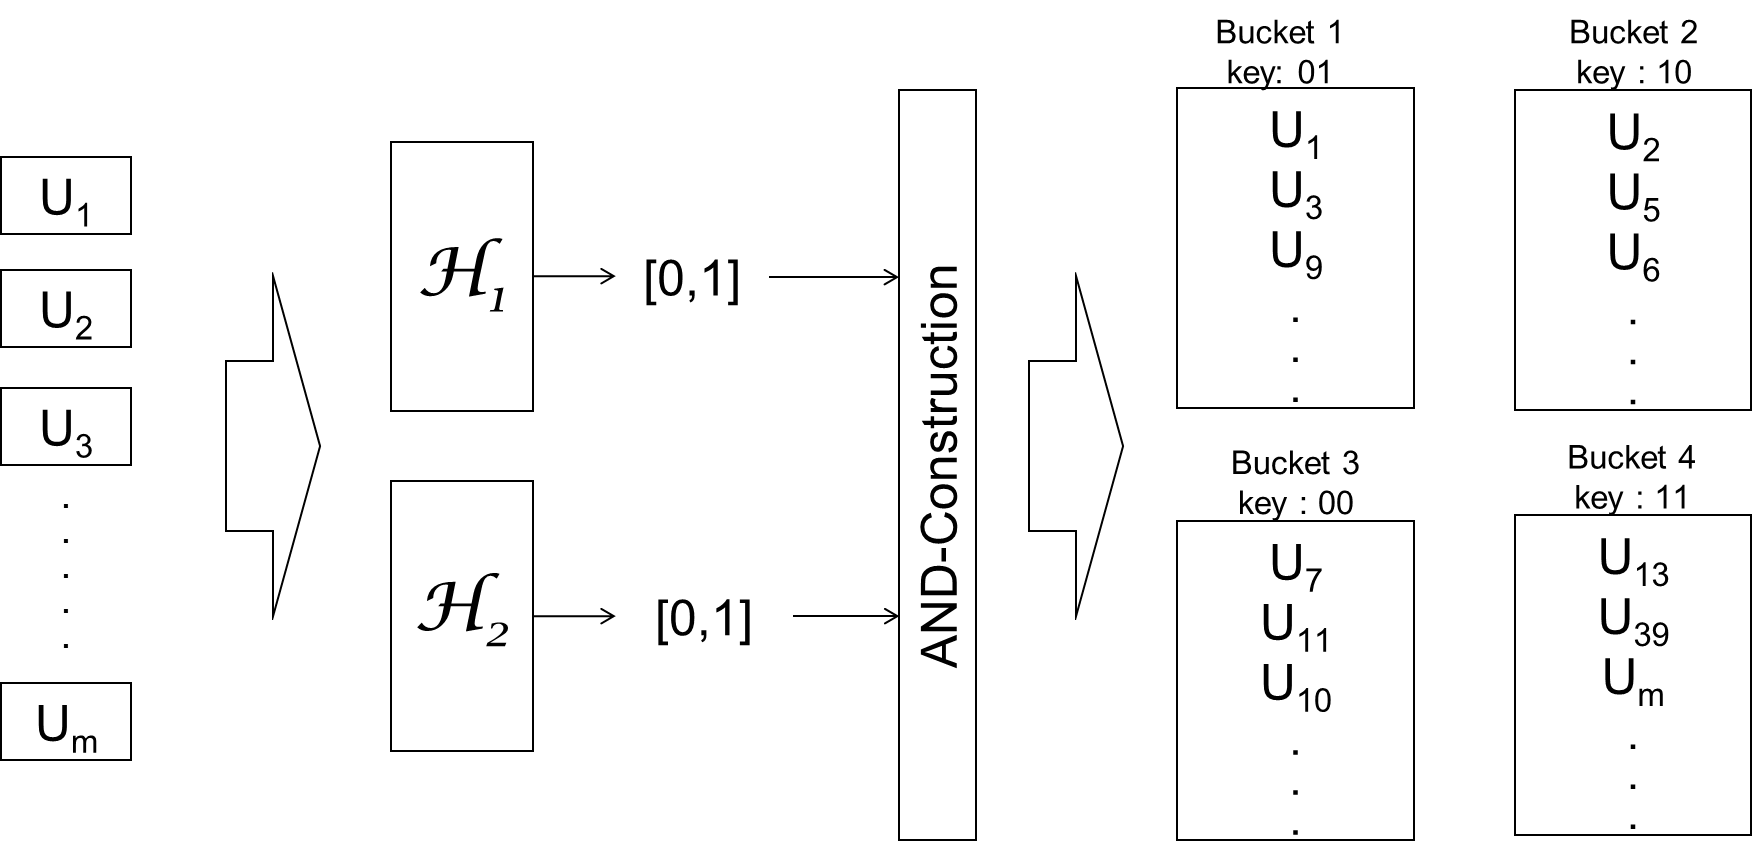
\includegraphics[scale=0.3]{lsh.png}
   \caption{Mapping user vectors ${U_1, U_2, ...., U_m}$ to the buckets of a\
   hash table via LSH using AND$-$Construction.}
   \label{fig:lsh-illustra}
\end{figure}


\section{LSH For Prediction}
\label{sec:lsh-prediction}
As described in Section \ref{sec:cf}, in neighborhood-based methods general 
approach is to investigate every user and item to find the most similar ones. 
Then the similar users or items are used to make a prediction. With LSH we can 
find the similar users or items without comparing every user or item with each other.
We can retrieve the similar items or users, called candidate pairs, to a target
item or user then compute the prediction with the retrieved candidate set. 
We can make a prediction of an items rating for a user with LSH as follows. For 
each hash table, we compute a hash key for the target user and retrieve the 
candidate users with the same hash key from the hash tables. if a candidate user
comes from multiple hash tables, we weight it with the number of hash tables 
it occurs call it frequency. Other wise all users treated equally weighted. Once we 
retrieved candidate sets from all hash tables, we take the union of all candidate 
sets and select the users who rated for the target item. Then we use their 
ratings, weighted with frequency, to compute the prediction for the target user.
Computational complexity of this method shown in Table \ref{table:complexity-lsh}.

Let $\hat{r}_{ui}$ is the rating of user $u$ on item $i$ that will be predicted.
We use following formula (Eq. \ref{eq:lsh-prediction}) to predict the ratings 
of user $u$ on the item $i$:
\begin{equation}
\hat{r}_{ui} = \frac{\sum\limits_{t=1}^{L} \sum\limits_{v \in C_i(t)} r_{vi}}{\sum\limits_{t=1}^{L} \mid C_i(t) \mid} ,
\label{eq:lsh-prediction}
\end{equation}
where; $L$ is the number of hash tables (bands) and  $C_i(t)$ is the set of 
candidate pairs who have rated for item $i$ retrieved from hash table $t$.

\begin{table}
\centering
\begin{tabular}{llll}
\hline
& & \multicolumn {2}{c}{Time} \\
\cline{3-4}
     & Space & Model Build  & Query \\
\hline
LSH & $O(|U||L|)$ & $O(|U|)$ &$O(|C||L|)$ \\
\hline
\end{tabular}
\caption{The space and time complexity of LSH  method, as a function of U, L, and C}
\label{table:complexity-lsh}
\end{table}

\section{Experiments}
\label{sec:experiements}

We evaluate collaborative filtering and LSH method in terms of the accuracy 
and efficiency. Experiments are carried out as follows. We first divided 
dataset, $R$, into two subset of training, $R_{train}$, and test, $R_{test}$ 
sets. We used the training data set to build LSH model. Then we evaluated LSH 
and CF algorithms on test data sets in terms of the prediction accuracy and
performance. For these experiments we used holdout cross validation. We holdout
\%5 of data set as test, $R_{test}$, \%5 of data set as validation, $R_{val}$, 
and used the rest as training data set, $R_{train}$, then run the experiments. 
We performed this experiment three times and averaged results over the rounds. 
We first run cross validation tests to detect optimum parameters $k$ and $Y$ on 
validation data sets. We then set these parameters and run the experiments on 
the test set to measure the performance of LSH and CF. We finally run tests to 
find out how the boundaries of LSH parameters effect accuracy and efficiency. 


\subsection{Data Sets}
MovieLens data set is used to train, test, and evaluate the system. Table 
\ref{table:data-set} shows the number of users, items and sparsity level of 
the data data.

\begin{table}[!ht]
\centering
\begin{tabularx}{0.45\textwidth}{XXXXX}
\hline
Data Set & Number of \newline Users & Number of \newline Items & Number of \newline Transactions & Sparsity \\
\hline
MovieLens     & 943	& 1682	  & 100000   & 0.0630   \\
\hline
\end{tabularx}
\caption{MovieLens data set used in the experiments.}
\label{table:data-set}
\end{table}


\subsection{Results}

We run parameter detection tests on validation data set first. We run CF user-based prediction tests for $k$ nearest neighbor parameter. In neighborhood based CF, $k$ number of neighbors is used for prediction calculations. We start $k$ from one and increased by five up to fifty and computed MAE as shown in Fig. \ref{fig:mae-k-ub}. We found out that for our data set user-based CF performs best when $k$ is around 30. We set $k$ to 30 and run another experiment to detect the optimum $Y$, significance, parameter. Fig. \ref{fig:mae-y-ub} shows that user-based CF performs best, in terms of accuracy, when $Y$ is around seven.
\begin{figure}
        %\centering
        \begin{subfigure}[b]{0.225\textwidth}
                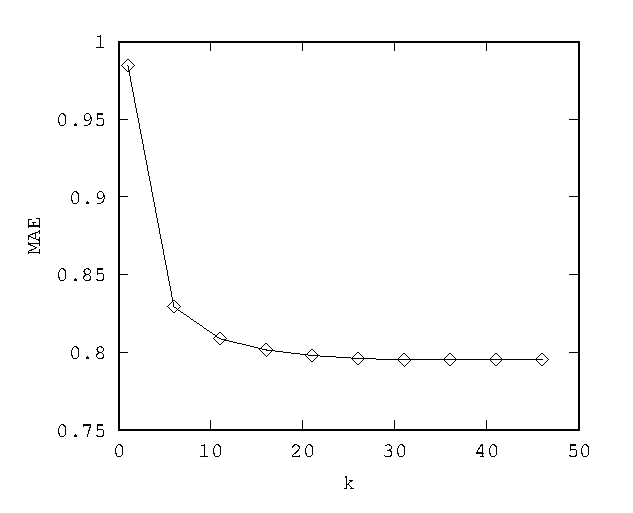
\includegraphics[width=\textwidth]{charts/ub-mae-k.eps}
                \caption{MAE and k}
                \label{fig:mae-k-ub}
        \end{subfigure}
        \quad
        \begin{subfigure}[b]{0.225\textwidth}
                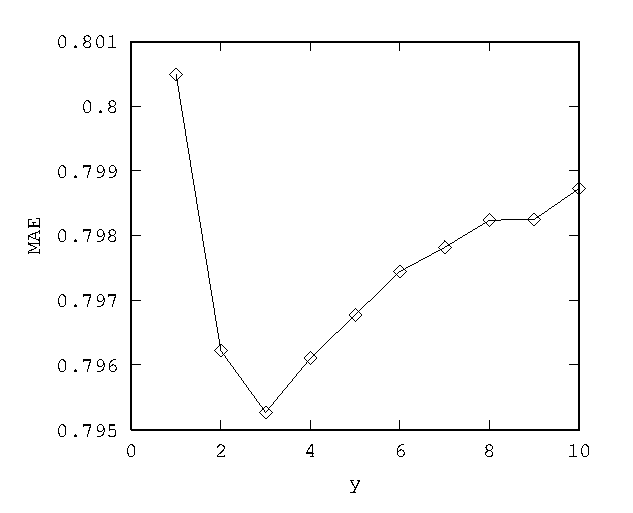
\includegraphics[width=\textwidth]{charts/ub-mae-y.eps}
                \caption{MAE and Y}
                \label{fig:mae-y-ub}
        \end{subfigure} 
        \caption{User-based CF accuracy against k, nearest neighbor, and Y, significance, parameters.}
        \label{fig:ub-parameters}
\end{figure}


With the optimum $k$ and $Y$,  we run the prediction tests on the test set for user-based CF. We found average MAE as 0.79527 and average running time as 9.437 seconds. We compare this results with the results of proposed LSH method.

We run 10x10 experiments to detect the effect of LSH parameters, number of hash tables and functions. Fig. \ref{fig:lsh-2d} shows the heat map figures of these experiments.

\begin{figure}
        %\centering
        \begin{subfigure}[b]{0.225\textwidth}
                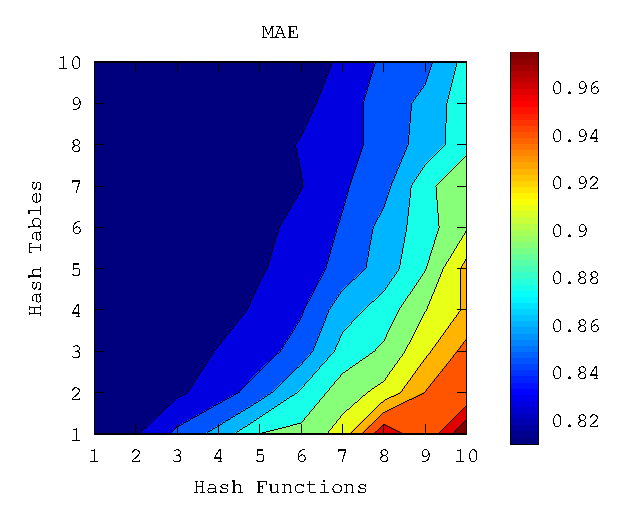
\includegraphics[width=\textwidth]{charts/mae-lsh-heat-map.eps}
                \caption{MAE}
                \label{fig:lsh-2d-mae}
        \end{subfigure}
        \quad
        \begin{subfigure}[b]{0.225\textwidth}
                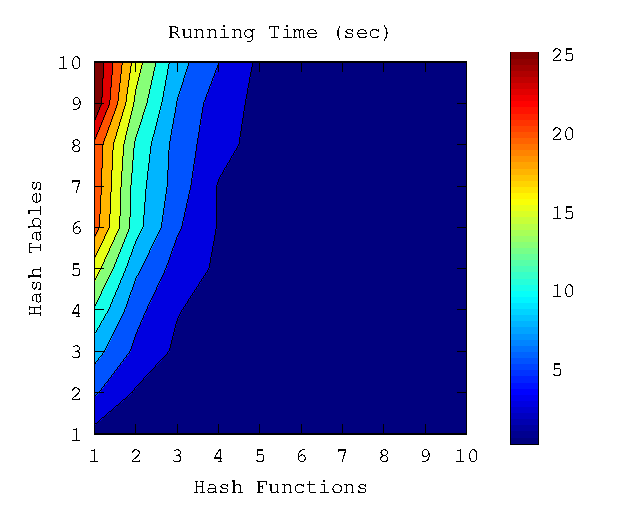
\includegraphics[width=\textwidth]{charts/runtime-lsh-heat-map.eps}
                \caption{Performance}
                \label{fig:lsh-2d-runtime}
        \end{subfigure} 
        \\
         \begin{subfigure}[b]{0.225\textwidth}
                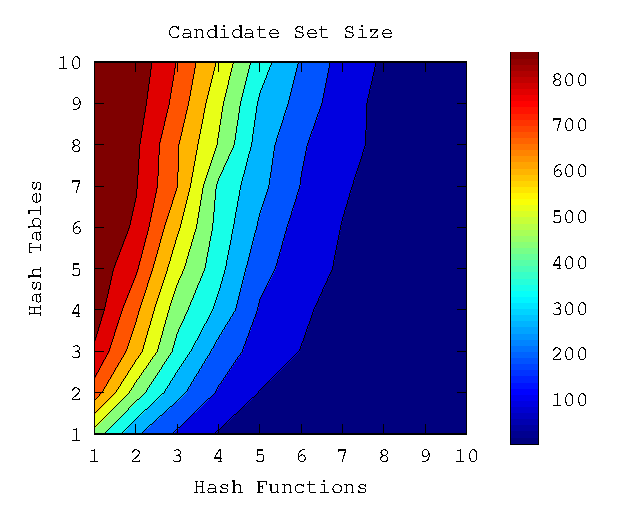
\includegraphics[width=\textwidth]{charts/candidate-set-lsh-heat-map.eps}
                \caption{Candidate Set Size}
                \label{fig:lsh-2d-candidate-size}
        \end{subfigure} 
        \caption{How accuracy and performance effected by Number of Hash Tables and Functions change in LSH.}
        \label{fig:lsh-2d}
\end{figure}

In order to show the effect of LSH parameters better, we draw heat map figures 
of hash functions and tables (Fig. \ref{fig:lsh-2d}). Note that increasing number 
of hash tables effects MAE in a better way (Fig. \ref{fig:ub-lsh-tables-mae}). 
This is because, increasing the number of tables reduces false negatives. On 
the other hand, when we increase the number of hash functions, MAE gets worse 
(Fig. \ref{fig:ub-lsh-functions-mae}), because, LSH selects only the most similar 
users and candidate set size, which is used for predictions, gets smaller, hence, 
false negatives are increased. As oppose to MAE, performance gets better when 
number of hash functions increase (Fig. \ref{fig:ub-lsh-tables-runtime}), because 
the candidate set size decreases (Fig. \ref{fig:lsh-tables-candidate-size}). 
In addition to decrease in candidate set size we eliminate the similarity 
computation with LSH prediction (\ref{eq:lsh-prediction}).

\begin{figure}[!h]
        %\centering
        \begin{subfigure}[b]{0.225\textwidth}
                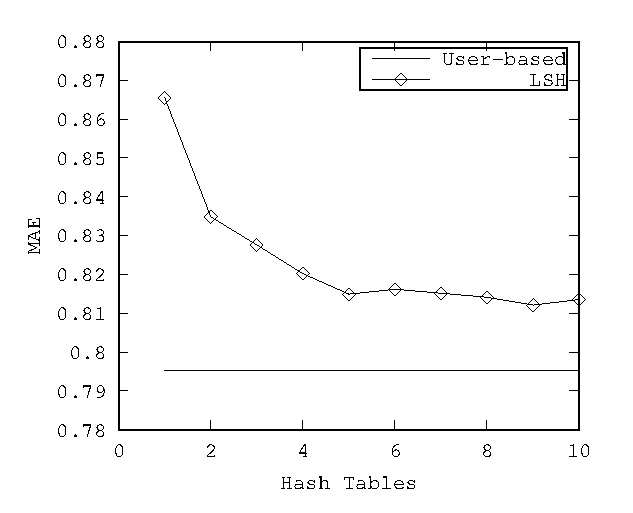
\includegraphics[width=\textwidth]{charts/ub-mae-hash-tables.eps}
                \caption{MAE}
                \label{fig:ub-lsh-tables-mae}
        \end{subfigure}
        \quad
        \begin{subfigure}[b]{0.225\textwidth}
                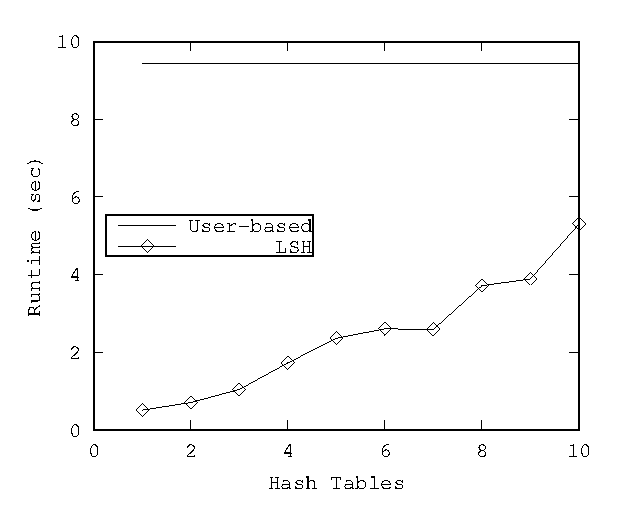
\includegraphics[width=\textwidth]{charts/ub-runtime-hash-tables.eps}
                \caption{Performance}
                \label{fig:ub-lsh-tables-runtime}
        \end{subfigure} 
        \\
         \begin{subfigure}[b]{0.225\textwidth}
                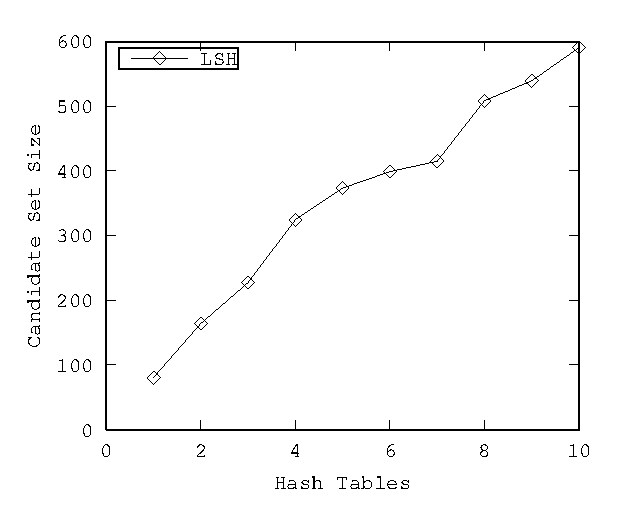
\includegraphics[width=\textwidth]{charts/lsh-canidate-hash-tables.eps}
                \caption{Candidate Set Size}
                \label{fig:lsh-tables-candidate-size}
        \end{subfigure} 
        \caption{User-based and LSH in terms of accuracy, performance, and hash tables.}
        \label{fig:ub-lsh-tables}
\end{figure}

We compare LSH method with user-based collaborative filtering in terms of hash 
functions and hash tables. 

Fig. \ref{fig:ub-lsh-tables} shows how the change of 
hash tables effect MAE and performance. As we said before, increasing number of 
hash tables increases the candidate set size (Fig. \ref{fig:lsh-tables-candidate-size}) 
and this reduces false negatives hence MAE is improved and got closer to the MAE in 
user-based method (Fig. \ref{fig:ub-lsh-tables-mae}). Even though MAE of LSH 
is still worse then user-based method, we gain a lot in terms of the performance 
(Fig. \ref{fig:ub-lsh-tables-runtime}).

\begin{figure}[!h]
        %\centering
        \begin{subfigure}[b]{0.225\textwidth}
                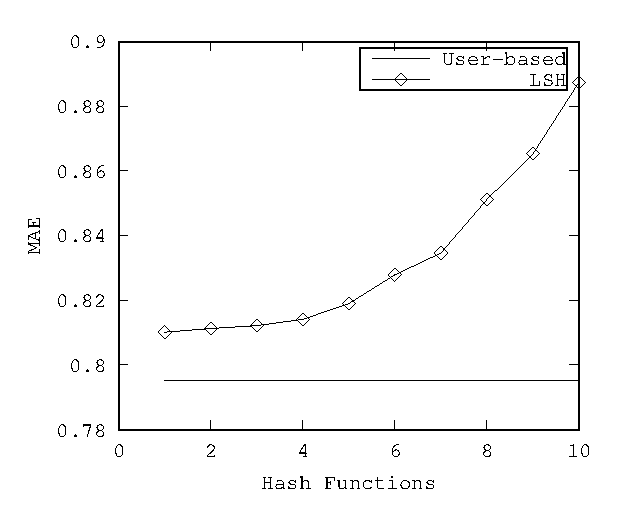
\includegraphics[width=\textwidth]{charts/ub-mae-hash-functions.eps}
                \caption{MAE}
                \label{fig:ub-lsh-functions-mae}
        \end{subfigure}
        \quad
        \begin{subfigure}[b]{0.225\textwidth}
                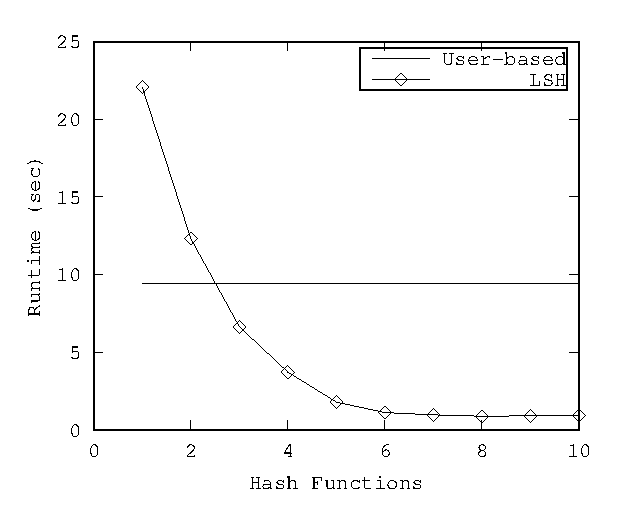
\includegraphics[width=\textwidth]{charts/ub-runtime-hash-functions.eps}
                \caption{Performance}
                \label{fig:ub-lsh-functions-runtime}
        \end{subfigure} 
        \\
         \begin{subfigure}[b]{0.225\textwidth}
                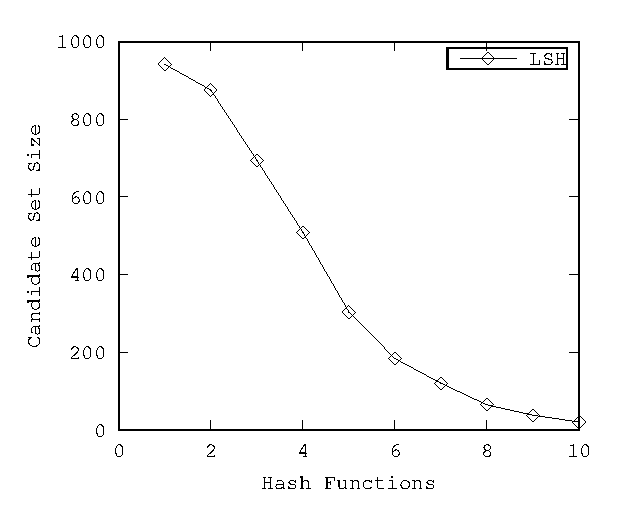
\includegraphics[width=\textwidth]{charts/lsh-canidate-hash-functions.eps}
                \caption{Candidate Set Size}
                \label{fig:lsh-functions-candidate-size}
        \end{subfigure} 
        \caption{User-based and LSH in terms of accuracy, performance, and hash functions.}
        \label{fig:ub-lsh-functions}
\end{figure}

Fig. \ref{fig:ub-lsh-functions} shows how the change of 
hash functions effects MAE and performance. As we said before, increasing number of 
hash functions decreases the candidate set size (Fig. \ref{fig:lsh-functions-candidate-size}) 
and this increases false negatives, hence, MAE gets worse (Fig. \ref{fig:ub-lsh-functions-mae}). 
Even though MAE of LSH gets worse then user-based method, we gain a lot in 
terms of the performance as we increase the number of hash functions (Fig. \ref{fig:ub-lsh-functions-runtime}). 

\begin{figure}[!h]
        %\centering
        \begin{subfigure}[b]{0.225\textwidth}
                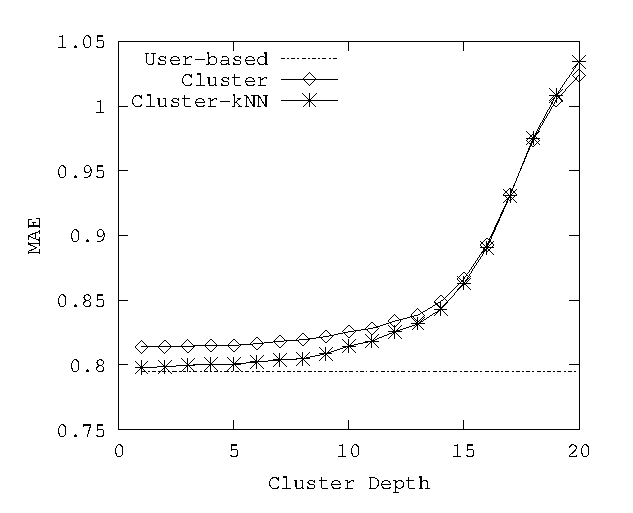
\includegraphics[width=\textwidth]{charts/cl-mae.eps}
                \caption{MAE}
                \label{fig:cl-mae}
        \end{subfigure}
        \quad
        \begin{subfigure}[b]{0.225\textwidth}
                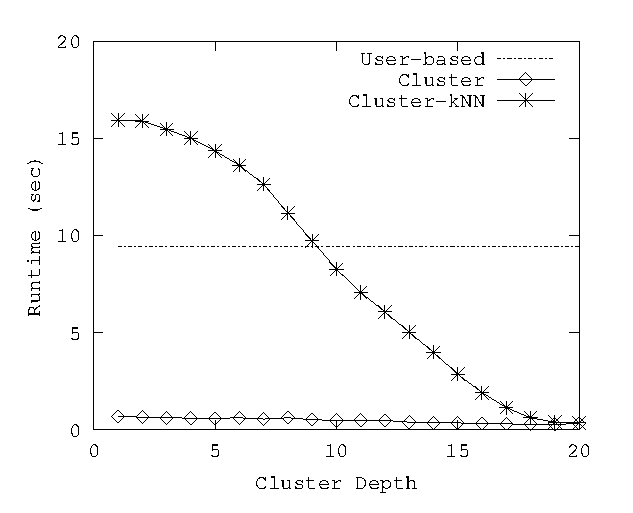
\includegraphics[width=\textwidth]{charts/cl-runtime.eps}
                \caption{Performance}
                \label{fig:cl-runtime}
        \end{subfigure} 
        \\
         \begin{subfigure}[b]{0.225\textwidth}
                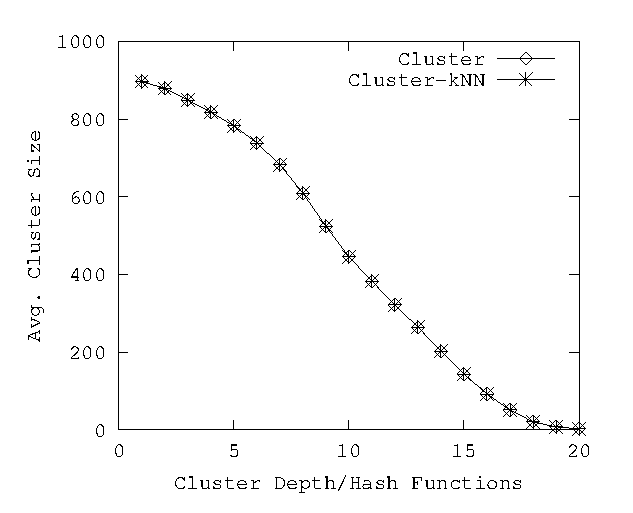
\includegraphics[width=\textwidth]{charts/cl-size.eps}
                \caption{Average Cluster Size}
                \label{fig:lsh-functions-candidate-size}
        \end{subfigure} 
        \caption{User-based, Clustering, and user-based with clustering results in terms of accuracy, performance, and cluster depth.}
        \label{fig:custering}
\end{figure}


\section{Conclusion}

In this term paper we have evaluated application of LSH to the prediction 
problem of recommendation and compared it against user-based neighborhood 
method of CF. 

We found out that proposed LSH calculation of the predictions tremendously 
improved the scalability of recommendation as appose to traditional CF methods 
and maintained the accuracy in acceptable ranges. Proposed LSH method performs 
worse, which is expected, then user-based CF method but gains a lot in performance.
This is because we eliminate the similarity calculation in order to make a prediction. 
We let LSH algorithm to find the similar users or items (candidate set) and compute 
the predictions by using this candidate set.

With different configuration parameters of LSH, we can get scalable and 
better results than user-based method. LSH model needs to be
configured to provide optimum outcome that balances MAE  and running time
according to the priorities of expectations from the system.

In order to complete the evaluation of this method in recommendation domain, 
we need to run more experiments to find out how it performs against the $top-N$ 
recommendation problem, which is one of the main problems in recommendation 
domains. We also need to study this algorithms in terms of other recommendation 
metrics such as diversity, novelty, serendipity, and aggregate diversity. 
Another important issue in recommendation domain is the stability of 
recommendation system. Stability of proposed method needs to be discussed and 
evaluated too. 

\bibliography{scalability}
\bibliographystyle{plain} 

% that's all folks
\end{document}


